\chapter{Iteración 3: Primer prototipo de Hardware} % (fold)
\label{cha:iteracion_3}


\section{Introducción} % (fold)
\label{it3:sec:introduccion}

En esta nueva iteración, realizaremos el circuito eléctrico de la plataforma, usando como base de diseño a la placa de desarollo utilizada en la iteración 2. Este nuevo circuito, lo formaran aquellas partes de la placa de desarrollo que utilicemos dentro de nuestra plataforma, y descartaremos aquellas que no participan.


%la primera placa que fue una verga. tenia el rs232, tenia 8 entradas, tenia la alimentacion separada de la entrada para la programacion del micro. osea podia alimentarse mediante el debugger o alimentacion externa. se adapto el diseño de la placa para poder programar el micro con el debugger de silicon labs. hay que tener en cuenta que nos basamos en el diseño hecho por silicon labs de la placa de desarrollo c8051f352 que teniamos en el lac. la vamos a haber construido en esta iteracion, y lo unico que llego a hacer fue conectarse con la ide. nada mas, el resto no anduvo nada. %

% section introduccion (end)

\section{Objetivo de la iteracion}

Establecer un diseño de circuito electronico para la plataforma, basandonos en la placa de desarrollo utilizada en la iteracion 2, construirlo, y verificar su funcionamiento.

\section{Requerimientos de la iteración} % (fold)
\label{it3:sec:requerimientos_de_la_iteracion}

Teniendo en cuenta los requerimientos principales de la plataforma y el objetivo principal de la iteración actual, conformamos la siguiente lista de requerimientos:

\begin{itemize}
\item Al circuito se le deberían poder conectar 8 entradas analógicas. (deriva de 1.1)
\item Al circuito se le deberían poder conectar 4 entradas de eventos digitales externos. (deriva de 1.3)
\item Las entradas analógicas deberían tener filtros para mejorar la inmunidad al ruido. (deriva de 2.2)
\item Se debería incluir en el diseño el circuito necesario para soportar comunicación vía RS232. (deriva de 1.6)
\item La placa debería poder alimentarse a través de una fuente de tensión externa. [3.1]
\item Se debería poder conectar el debugger del microcontrolador a la placa para poder programarlo. [3.2]
\end{itemize}


% section requerimientos_de_la_iteracion (end)

\section{Desarrollo} % (fold)
\label{it3:sec:desarrollo}

\subsection{Elección de Herramientas para Diseño} %(fold)
\label{it3:sub:herramientas_para_diseno}

Las herramientas de diseño fueron elegidas basándonos en experiencias de otros alumnos e ingenieros en el Laboratorio de Arquitectura de Computadoras. En particular, el ingeniero Santiago Rodriguez, nos aconsejo utilizar una de las siguientes herramientas:

\begin{itemize}
\item Kicad.
\item Altium Designer.
\item Eagle.
\item PCBwizard.
\end{itemize}

La impresión del PCB se realizo utilizando una maquina fresadora perteneciente al laboratorio, modelo ProtoMat E33 de LPKF. Para realizar una impresión, era necesario instalar el programa LPKF Circuit en un ordenador.

La herramienta de diseño que mas se ajusto a nuestras necesidades fue Kicad, debido principalmente a su sencillez, y su facilidad para exportar archivos en el formato correcto para la maquina fresadora.

%subsection herramientas_para_diseno (end)

\subsection{Diagramas de Bloques de Hardware}
\label{it3:sub:diagrama_de_bloques_de_hardware}

La primera etapa de diseño consistió en realizar un diagrama de bloques que, en base a los requerimientos planteados para esta iteración, ilustre a grandes rasgos la organización del circuito que pretendemos realizar. \\

\begin{figure}[h]
  \centering
  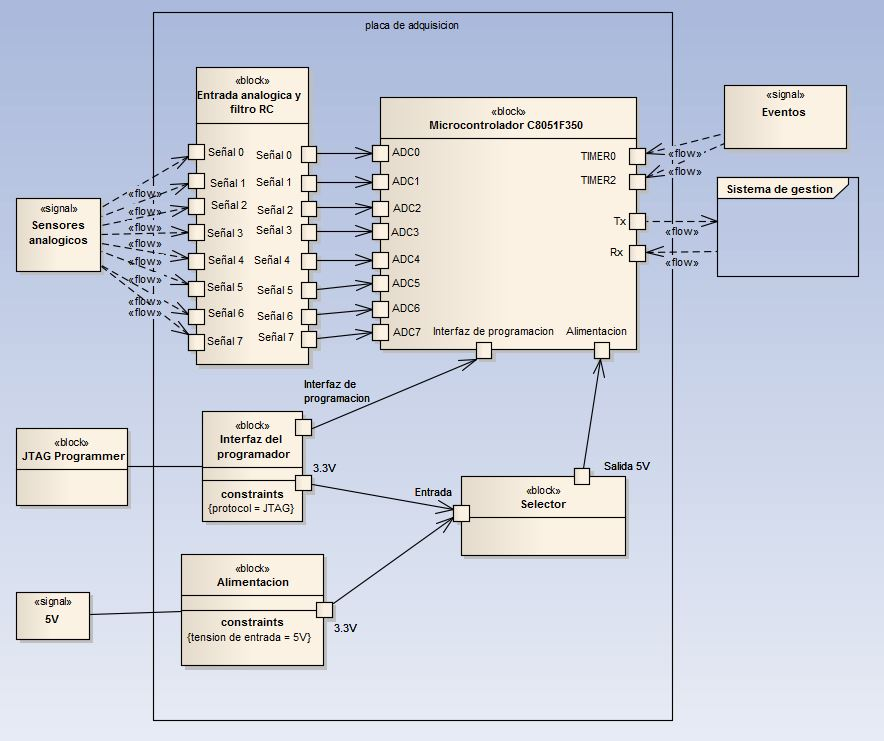
\includegraphics[width=1\textwidth, height = 12cm]{BloquesHardw1}
  \caption{Diagrama de Bloque de la Plataforma.}\label{fig:BloquesHardw1}
\end{figure}

Los bloques en la Figura \ref{fig:BloquesHardw1} representan de forma general los distintos módulos a implementar. Las entradas analógicas se introducen al microcontrolador a través de filtros RC (reductores del ruido), para luego pasar al conversor analógico-digital. El bloque GPIO (Entrada/Salida de propósito general) consiste en un grupo de pines direccionados a distintas entradas del microcontrolador. Estos pines pueden tener funcionalidades generales, y algunos pueden tener otras mas especificas, como ser: contador de eventos, PCA, PWM, etc. En nuestro diseño, separamos aquellos pines específicos que se utilizan como contadores de eventos, y además agregamos 4 pines de propósito general, por la eventual necesidad de requerirlos. \\

La alimentación del sistema puede ser suministrada de dos formas posibles: Mediante una fuente de tensión externa de 5V, o por el mismo debugger del microcontrolador. Por la posible necesidad de programar mas de una vez el microcontrolador, decidimos colocar una llave selectora que permite seleccionar la entrada de alimentación. Por lo que es posible alimentarlo de ambas formas. 

%subsection diagra_bloques_hardware (end)

\subsection{Diseño Esquemático}
\label{it3:sub:diseno_esquematico}

El diseño esquemático del circuito fue realizado con la herramienta de software KiCad. Para facilitar la descripción, seccionamos el circuito final en múltiples circuitos, y los elaboraremos por separado, para luego mostrar el circuito final.

\subsubsection{Entradas Analógicas}
\label{it3:ssub:entradas_analogicas}

Cada una de las 8 entradas analógicas tienen circuitos de conexión similares. La Figura \ref{fig:esquematicoFiltro} ilustra el circuito para una de estas entradas. \\

El ruido en el sistema es un factor importante a tener en cuenta. Ingresa por interferencia de señales externas, por temperatura, por la fuente de tensión, y por los mismos componentes que conforman el circuito. Como primera medida, cada entrada analógica contiene un filtro RC pasivo que reduce el ruido en una primera instancia. Además, el mismo microcontrolador trata el ruido de la señal para mejorar la relación SNR. \\

En la Figura \ref{fig:esquematicoFiltro} se muestra un pin de entrada AI0, que se conecta a la salida de un dispositivo de instrumentación. La señal de este sensor, se filtra mediante el circuito RC compuesto por una resistencia de 100 Ohms y un capacitor de 0,1 $\mu$F.

\begin{figure}[H]
  \centering
  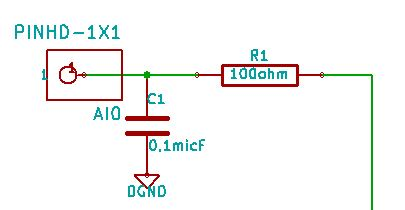
\includegraphics[width=0.70\textwidth, height = 4cm]{esquematicoFiltro}
  \caption{Esquemático del circuito de entrada analógica, más filtro RC pasa-bajo.}\label{fig:esquematicoFiltro}
\end{figure}

%subsubsection entradas_analogicas (end)

\subsubsection{Circuito de interfaz serial}
\label{it3:ssub:circuito_de_interfaz_serial}

La interfaz serial RS-232 es necesaria para el acondicionamiento del canal de datos entre la plataforma y el sistema embebido de destino. En esta sección elaboramos la construcción del circuito de dicha interfaz. \\

La salida serial del microcontrolador tiene un nivel de tensión TTL, insuficiente para un adaptador RS-232, por lo que fue necesario adaptar este nivel para asegurar el correcto envío de datos. El circuito de adaptación se muestra en la Figura \ref{fig:esquematicoMax232}. Contiene un integrado MAX232 que es utilizado ampliamente en la industria para adaptar niveles TTL a RS-232. Los pines "XRX1", "XCTS1", "XTX1" y "XRTS1" son los correspondientes al modulo de salida del adaptador serial. \\

Además de la adaptación, colocamos 4 jumpers (JP1, JP2, JP3, JP4) a la entrada del integrado MAX232 en caso en que se requiera la salida TTL del microcontrolador. \\

\begin{figure}[H]
  \centering
  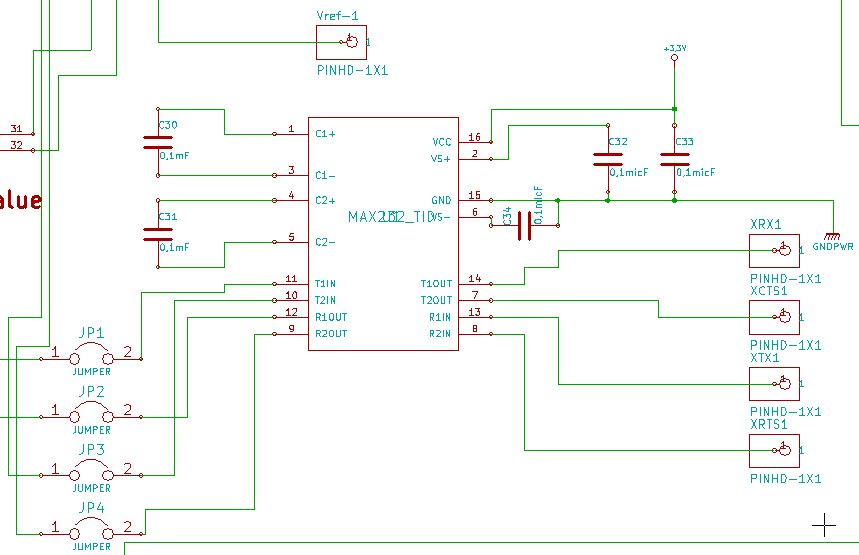
\includegraphics[width=1.0\textwidth, height = 8cm]{esquematicoMax232}
  \caption{Esquemático del Circuito MAX232 .}\label{fig:esquematicoMax232}
\end{figure}

%subsubsection salida_serial (end)

\subsubsection{Circuito de alimentación}
\label{it3:ssub:circuito_de_alimentacion}

La tensión de alimentación del circuito de la plataforma es de 3,3V. Con el propósito de utilizar una fuente de alimentación genérica de 5V, utilizamos un regulador de tensión LM2937 que baja de un nivel de 5V a 3,3V.

Es posible alimentar el circuito mediante una fuente de 5V o el debugger del mismo microcontrolador. Este debugger entrega 3,3V a la salida, por lo que, si el debugger esta conectado como alimentación, no es necesario utilizar el regulador de tensión.

La Figura \ref{fig:esquematicoPotencia} muestra el circuito de alimentación. Colocamos una serie de jumpers que permiten seleccionar si se alimentara el circuito con una fuente de 5V, o el debugger del microcontrolador

\begin{figure}[H]
  \centering
  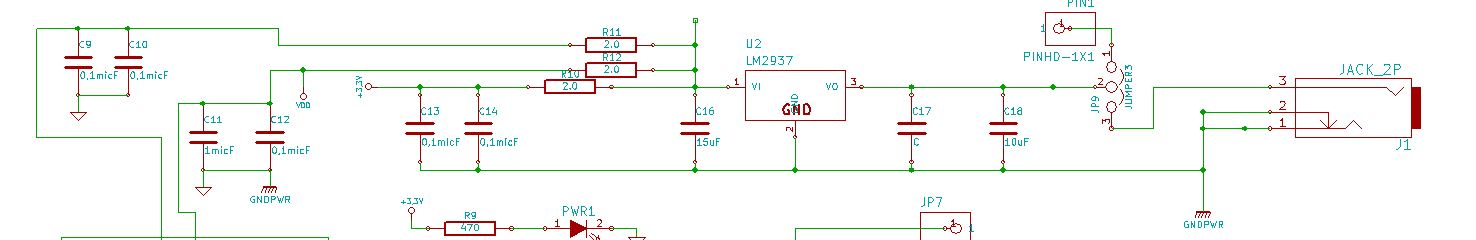
\includegraphics[width=1.0\textwidth, height = 6cm]{esquematicoPotencia}
  \caption{Esquemático del Circuito de Potencia.}\label{fig:esquematicoPotencia}
\end{figure}

%Para poder alimentar al microcontrolador necesitábamos 3.3V así que utilizamos un regulador de tensión (LM2937). El C8051f352 tiene dos entradas de alimentación, una analógica y una digital, ambas con un rango entre 2.9V a 3.6V, ademas la corriente puede variar entre 5.7mA (en estado inactivo) hasta 11.3mA (en estado activo). Es por ello que se colocan las resistencias, y ademas se colocan capacitores en paralelo para disminuir el ruido de entrada.

%subsubsection circuito_potencia (end)

\subsubsection{Diagrama Esquemático Final}
\label{it3:ssub:diagrama_esquematico_final}

De los circuitos descritos anteriormente, se ilustra el circuito final en la Figura \ref{fig:EsquematicoCompleto1}

\begin{figure}[H]
\centering
  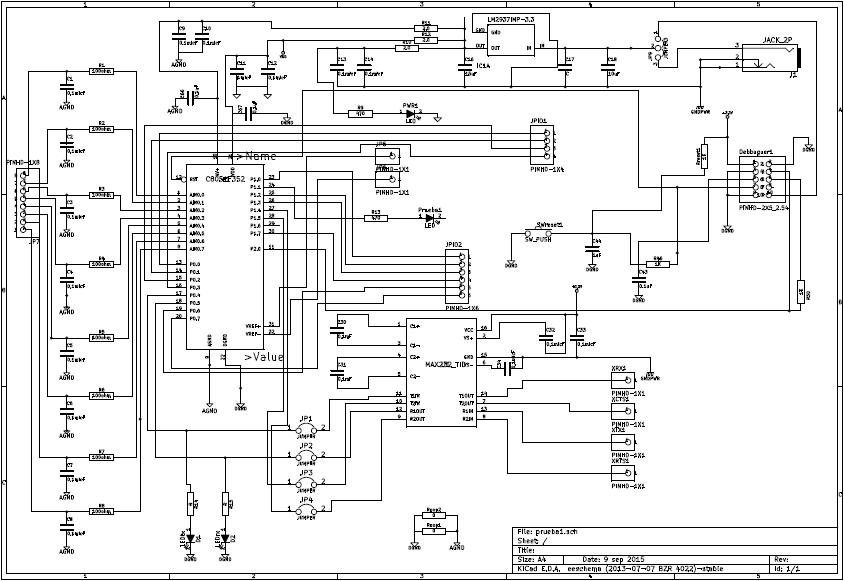
\includegraphics[width=1\textwidth, height = 11cm]{EsquematicoCompleto1}
  \caption{Esquemático del Circuito Completo de la placa.}\label{fig:EsquematicoCompleto1}
\end{figure}

%subsubsection esquematico_final_1 (end)

%subsection diseno_esquematico (end)

\subsection{Impresión de circuito en placa de cobre}
\label{it3:sub:impresion_de_circuito_en_placa_de_cobre}

Una plaqueta de circuito impreso (PCB) es una superficie constituida por caminos o pistas de material conductor, laminadas sobre una base no conductora. El circuito que se imprime en un plaqueta se utiliza para interconectar distintos dispositivos electrónicos.

En el Laboratorio de Arquitectura de Computadoras, donde fue realizado este proyecto, esta disponible una maquina fresadora con control numérico por computadora, para la impresión de placas PCB, modelo LPKF E33. El PCB diseñado fue impreso con esta maquina. El software utilizado para la impresión fue ``Circuit Pro'', proveído por los mismos fabricantes de la maquina fresadora. 

La Figura \ref{fig:PCB1} ilustra la proyección de componentes en el PCB, antes de ser impreso.

\begin{figure}
\centering
  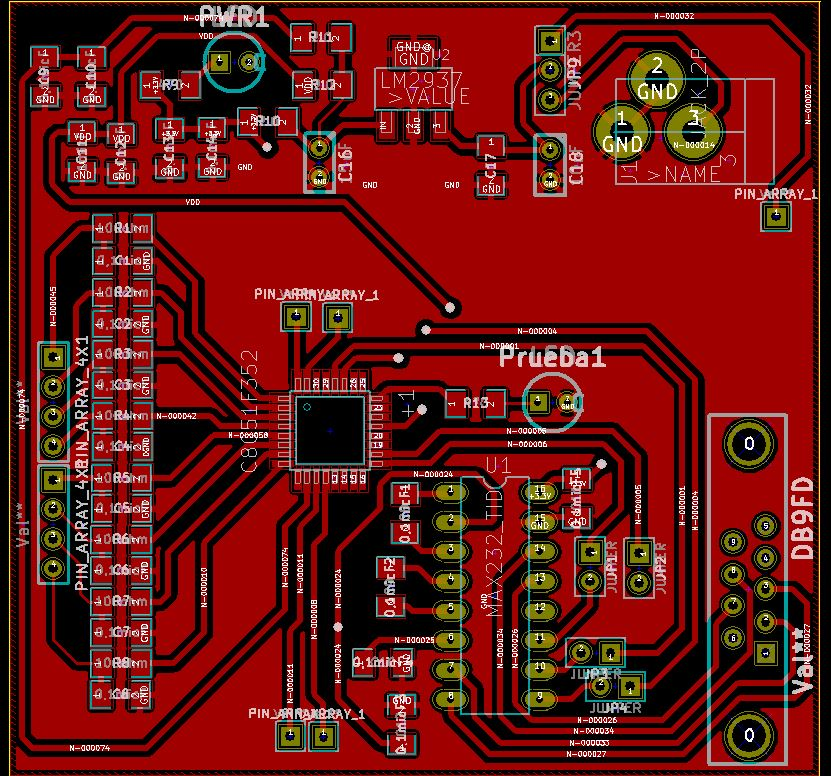
\includegraphics[width = 0.70\textwidth, height = 9cm]{PCB1}
  \caption{Despliegue de componentes en el circuito impreso}\label{fig:PCB1}
\end{figure}


%subsection pcb1 (end)

% section desarrollo (end)

\clearpage


\section{Pruebas} % (fold)
\label{it3:sec:pruebas}


\begin{table}[h]
\caption{Test de sistema 1: Correcto Diseño de PCB}
\label{it3:tab:testsistema1}
\begin{tabular}{p{2cm} p{9cm}}
\multicolumn{2}{c}{\cellcolor[HTML]{68CBD0}{\color[HTML]{000000} Prueba de sistema}} \\                                  
Prueba \#        & 1 \\
\hline
Nombre           & Correcto Diseño de PCB. \\ 
\hline
Requerimientos &   1.1, 1.3, 1.6, 2.2 \\
\hline
Descripción      & Se chequea si existen errores en el diseño utilizando el proceso ERC (perfom design rules check), proveido por el software KiCad. \\
\hline
Pre-condiciones  & \tabitem Componentes colocados y sus rutas de pistas establecidas. \\
                 & \tabitem Pads numerados con sus etiquetas.  \\
\hline
Post-condiciones & El resultado de ERC debe ser cero. \\
\hline
Resultados       & No encontramos errores de diseño en el PCB.                                                                                       
\end{tabular}
\end{table}

\begin{table}[h]
\caption{Test de sistema 2: Correcta impresión de la placa.}
\label{it3:tab:testsistema2}
\begin{tabular}{p{2cm} p{9cm}}
\multicolumn{2}{c}{\cellcolor[HTML]{68CBD0}{\color[HTML]{000000} Prueba de sistema}} \\
Prueba \#        & 2 \\
\hline
Nombre           & Correcta impresión de la placa. \\
\hline
Requerimientos &   1.1, 1.3, 1.6, 2.2  \\                                                                                                                                                              
\hline
Descripción      & Corroboramos que todas las pistas y que todos los esquemas de perforado se hayan impreso correctamente. Luego, con un multímetro en modo continuidad, comprobamos que no existan cortocircuitos entre pistas y masa o entre pads y masa. \\
\hline
Pre-condiciones  & \tabitem Placa impresa. \\
                 & \tabitem Multímetro en modo de medición por continuidad.\\
\hline

Post-condiciones & La placa debe tener las mismas pistas que aparecen en el diseño de PCB, y al medir con el multímetro nunca debe dar continuidad entre masa y pistas, o entre pads y pistas. \\
\hline
Resultados       & Todas las pistas se correspondían con el diseño de PCB. Pero, al medir la continuidad de las pistas, se encontraron algunos cortocircuitos producidos por una mala colocación de la plancha al momento de la impresión. Los resultados de esta prueba obligaron a reiteradas impresiones del PCB, hasta que esta prueba de los resultados esperados. \\
\end{tabular}
\end{table}

\begin{table}[h]
\centering
\caption{Test de sistema 3: Correcta soldadura de Componentes}
\label{it3:tab:testsistema3}
\begin{tabular}{p{2cm} p{9cm}}
\multicolumn{2}{c}{\cellcolor[HTML]{68CBD0}{\color[HTML]{000000} Prueba de sistema}} \\
Prueba \#        & 3 \\
\hline
Nombre           & Correcta soldadura de Componentes \\
\hline
Requerimiento &   1.1, 1.3, 1.6, 2.2 \\

\hline
Descripción      & Se utiliza el multímetro en modo continuidad para poder comprobar si existen cortocircuitos y verificar si todos los componentes están bien interconectados. \\
\hline
Pre-condiciones  & \tabitem Placa impresa. \\
                 & \tabitem Pistas impresas correctamente. \\
                 & \tabitem Componentes soldados. \\
                 & \tabitem Multímetro en modo continuidad. \\
\hline 
Post-condiciones &  No debería haber cortocircuitos, y la interconexión entre los distintos componentes debería corresponderse con el diseño de PCB. \\ 
\hline
Resultados       & Luego de soldar los componentes, se encontraron algunos cortocircuitos presentes en la placa. Con la intención de arreglarlos, se estropearon algunas pistas, por lo que fue necesario imprimir la placa nuevamente y volver a soldar los componentes hasta que esta prueba dio los resultados esperados. \\
\end{tabular}
\end{table}

\begin{table}[h]
\centering
\caption{Test de sistema 4: Correcta Comunicación Con SiliconLabs Debugger.}
\label{it3:tab:testsistema4}
\begin{tabular}{p{2cm} p{9cm}}
\multicolumn{2}{c}{\cellcolor[HTML]{68CBD0}{\color[HTML]{000000} Prueba de sistema}} \\
Prueba \#        & 4 \\
\hline
Nombre           & Correcta Comunicación Con SiliconLabs Debugger. \\
\hline
Requerimiento &   3.2 \\                                                                         
\hline
Descripción      & Se utilizo el cable USB con el debugger de SiliconLabs para conectar la placa a la PC. \\
\hline
Pre-condiciones  & \tabitem Placa impresa. \\
                 & \tabitem Pistas impresas correctamente. \\
                 & \tabitem Componentes soldados. \\
                 & \tabitem IDE SiliconLabs instalada en la PC. \\
\hline
Post-condiciones &  Luego de intentar conectar el software con la placa a través del debugger, debería aparecer una notificación de que la placa esta exitosamente conectada al ordenador, y esta lista para ser programada. \\
\hline
Resultados       &  Conectamos la placa a un ordenador, y en la IDE de Silicon Labs, presionamos el botón de conectar. Luego de esto, apareció la notificacion que indicaba que el microcontrolador estaba exitosamente conectado al software de Silicon Labs.
\end{tabular}
\end{table}

\begin{table}[h]
\centering
\caption{Test de sistema 5: Correcta programación del microcontrolador.}
\label{it3:tab:testsistema5}
\begin{tabular}{p{2cm} p{9cm}}
\multicolumn{2}{c}{\cellcolor[HTML]{68CBD0}{\color[HTML]{000000} Prueba de sistema}} \\
Prueba \#        & 4 \\
\hline
Nombre           & Correcta programación del microcontrolador. \\
\hline
Requerimiento &   3.2 \\
\hline
Descripción      & Utilizando el debugger conectado a la PC, se intenta programar el microcontrolador con un programa de prueba, y verificarlo con la notificación del software que indique que se programo correctamente. \\
\hline
Pre-condiciones  & \tabitem Placa conectada al debugger \\
                 & \tabitem Debugger conectado a la PC via USB. \\
                 & \tabitem IDE SiliconLabs instalada en la PC. \\
                 & \tabitem C8051f352 reconocido por el software. \\
\hline

Post-condiciones &  Al intentar programar el microcontrolador utilizando la IDE, debería devolver una notificación, indicando su correcta programación. \\
\hline
Resultados       &  Conectamos la placa a la PC y en la IDE al intentar cargar el programa, devolvió un error de escritura de la flash del microcontrolador. La naturaleza de este error no fue evidente al principio, pero luego de investigar y con la ayuda del ingeniero Gustavo Parlanti, descubrimos que el problema se originaba en un ferrite conectado a la alimentación del microcontrolador. Para solucionar este problema, fue necesario rehacer la placa nuevamente.
\end{tabular}
\end{table}




% section pruebas (end)

\section{Conclusiones} % (fold)
\label{it3:sec:conclusiones}
La Figura \ref{fig:resultadohardware1} muestra el resultado final de la construcción en PCB de la plataforma.

\begin{figure}[h]
  \centering
  \includegraphics[width=0.80\textwidth, height = 10cm]{resultadohardware1}
  \caption{Placa completa con todo sus componentes soldados.}\label{fig:resultadohardware1}
\end{figure}

En esta iteración cumplimos con los siguientes requerimientos planteados:
\begin{itemize}
  \item Al circuito se le deben poder conectar 8 entradas analógicas. (deriva de 1.1)
  \item Al circuito se le deben poder conectar 4 entradas de eventos digitales externos. (deriva de 1.3)
  \item Las entradas analógicas deben tener filtros para mejorar la inmunidad al ruido. (deriva de 2.2)
  \item Se deberia incluir en el diseño el circuito necesario para soportar comunicación vía RS232. (deriva de 1.6)
  \item La placa debería poder alimentarse a través de una fuente de tensión externa. [3.1]
  \item Se debería poder conectar el debugger del microcontrolador a la placa para poder programarlo. [3.2]
\end{itemize}

Viendo los resultados de las pruebas, puede verse que no fueron una sino varias las veces que fue necesario reimprimir la placa, hasta lograr que funcionara como era esperado. En cada nueva impresión, se mejoraban aspectos relacionados a su tamaño, la distribución de los componentes, y su robustez con respecto a los posibles cortocircuitos generados a partir de imperfecciones en el ruteo de pistas.

% section resultados (end)

% chapter iteracion_3 (end)